\documentclass{standalone}
\usepackage{pgfplots}
\pgfplotsset{compat=newest}
\begin{document}
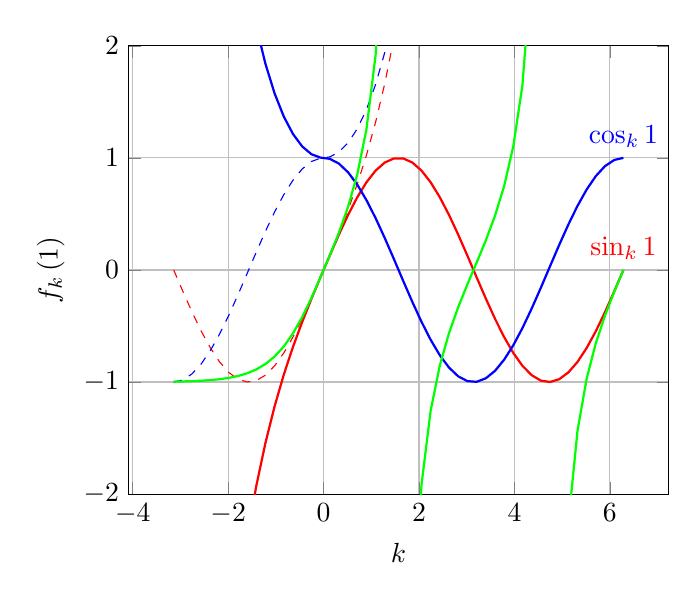
\begin{tikzpicture}[
        declare function={
                sine(\x)= (\x>=0) * sin(deg(\x)) + (\x<0) * sinh(\x);
            },
        declare function={
                cosine(\x)= (\x>=0) * cos(deg(\x)) + (\x<0) * cosh(\x);
            },
        declare function={
                tangent(\x)= (\x>=0) * tan(deg(\x)) + (\x<0) * tanh(\x);
            },
    ]
    \begin{axis}[
            xlabel = $k$,
            ylabel = $f_k\left(1\right)$,
            domain = -pi:+2*pi,
            ymin = -2,
            ymax = +2,
            restrict y to domain = -10:+10,
            grid = major,
            samples = 50,
        ]
        \addplot[
            color=red,
            dashed,
        ]{-sine(-x)};
        \addplot[
            color=blue,
            dashed,
        ]{cosine(-x)};
        \addplot[
            color=red,
            thick
        ]{sine(x)}node[above]{$\sin_k{1}$};
        \addplot[
            color=blue,
            thick
        ]{cosine(x)}node[above]{$\cos_k{1}$};
        \addplot[
            color=green,
            thick
        ]{tangent(x)};
    \end{axis}
\end{tikzpicture}
\end{document}